\documentclass[12pt,fleqn,handout]{beamer}


\xdefinecolor{lavendar}{rgb}{0.8,0.6,1}
\xdefinecolor{olive}{cmyk}{0.64,0,0.95,0.4}
%\xdefinecolor{olive}{cmyk}{1,0,0,0}
\xdefinecolor{mag}{cmyk}{0.1,1,0,0.2}
\xdefinecolor{lblue}{rgb}{0,0,1.5}
\xdefinecolor{lred}{rgb}{1,0,0}
\xdefinecolor{mine}{cmyk}{1,0,0.2,0}
\xdefinecolor{bluel}{cmyk}{0.1,0,0.9,0.4}

\usepackage{amsmath,amssymb,dsfont,mathrsfs}
\usepackage{tikz,pgflibraryplotmarks}
\usepackage{multimedia}
\usepackage{wasysym}
\usepackage{rotating}
\usepackage{algorithm,algorithmic}
\usepackage{graphicx} % more modern
\usepackage{subfigure}
\usepackage{booktabs}

\usepackage{pgfplots}
\usepackage{verbatim}

\usepackage{setspace}
\newlength\iwidth
\newlength\iheight

\newcommand\makebeamertitle{\frame{\maketitle}}%
\graphicspath{{./images/}}
\setbeamertemplate{navigation symbols}{}
\addtobeamertemplate{navigation symbols}{}{%
    \usebeamerfont{footline}%
    \usebeamercolor[fg]{footline}%
	\insertshorttitle
    \;--
    \insertframenumber
}

\newcommand{\sectionstart}{
	\only<beamer>{
 	\begin{frame}% (fold)
 		\begin{centering}\Huge \insertsection \par\end{centering}
 	\end{frame}% frame the_application (end)
	}
 }


% make bibliography entries smaller
\usepackage{natbib}
\setbeamertemplate{bibliography item}{[\theenumiv]}
\renewcommand\bibfont{\scriptsize}
\setbeamertemplate{frametitle continuation}[from second]
\newcommand{\tcr}{\textcolor{red}}
\newcommand{\tcrd}{\textcolor{red}}
\newcommand{\tcb}{\textcolor{bluel}}
\newcommand{\tcm}{\textcolor{mag}}
\newcommand{\tcg}{\textcolor{olive}}

\newcommand{\R}{\mathbb{R}}
\newcommand{\C}{\mathbb{C}}

% bold lower-case for vectors
\newcommand{\bfa}{{\bf a}}
\newcommand{\bfb}{{\bf b}}
\newcommand{\bfc}{{\bf c}}
\newcommand{\bfs}{{\bf s}}
\newcommand{\bfm}{{\bf m}}
\newcommand{\bfd}{{\bf d}}
\newcommand{\bfe}{{\bf e}}
\newcommand{\bfu}{{\bf u}}
\newcommand{\bfy}{{\bf y}}
\newcommand{\bfx}{{\bf x}}
\newcommand{\bfh}{{\bf h}}
\newcommand{\bfw}{{\bf w}}
\newcommand{\bfv}{{\bf v}}
\newcommand{\bfr}{{\bf r}}
\newcommand{\bfz}{{\bf z}}
\newcommand{\bfp}{{\bf p}}


% bold upper-case for linear operators
\newcommand{\bfA}{{\bf A}}
\newcommand{\bfB}{{\bf B}}
\newcommand{\bfZ}{{\bf Z}}
\newcommand{\bfM}{{\bf M}}
\newcommand{\bfC}{{\bf C}}
\newcommand{\bfD}{{\bf D}}
\newcommand{\bfQ}{{\bf Q}}
\newcommand{\bfJ}{{\bf J}}
\newcommand{\bfG}{{\bf G}}
\newcommand{\bfI}{{\bf I}}
\newcommand{\bfP}{{\bf P}}
\newcommand{\bfK}{{\bf K}}
\newcommand{\bfY}{{\bf Y}}
\newcommand{\bfW}{{\bf W}}
\newcommand{\bfR}{{\bf R}}
\newcommand{\bfL}{{\bf L}}
\newcommand{\bfF}{{\bf F}}
\newcommand{\bfT}{{\bf T}}
\newcommand{\bfS}{{\bf S}}
\newcommand{\bfX}{{\bf X}}
\newcommand{\bfU}{{\bf U}}
\newcommand{\bfV}{{\bf V}}
\newcommand{\bfH}{{\bf H}}


\newcommand{\calF}{\mathcal{F}}



\newcommand{\hf}{{\frac 12}}
\newcommand{\bftheta}{{\boldsymbol \theta}}
\newcommand{\bfxi}{{\boldsymbol \xi}}

\newcommand{\bfLambda}{{\boldsymbol \Lambda}}
\newcommand{\bfSigma}{{\boldsymbol \Sigma}}
\newcommand{\bfepsilon}{{\boldsymbol \epsilon}}

\newcommand{\E}{\vec E}
\newcommand{\B}{\vec B}

\newcommand{\vu}{  {\vec {\bf u}}}

\newcommand{\grad}{  {\vec {\bf \nabla}}}

\newcommand{\lfrownie}{\textcolor{red}{\large{\frownie}}}
\newcommand{\lsmiley}{\textcolor{green}{\large{\smiley}}}

\newcommand{\curl}{\ensuremath{\nabla\times\,}}
\renewcommand{\div}{\nabla\cdot\,}
\newcommand{\divh}{\nabla_h\cdot\,}
\renewcommand{\grad}{\ensuremath{\nabla}}

\DeclareMathOperator*{\argmin}{arg\,min}


\title[OC]{Optimal Control}
\subtitle{Numerical Methods for Deep Learning}
\date{}
\begin{document}

\makebeamertitle

\section{Optimization Problem} % (fold)
\label{sec:optimization_problem}
\begin{frame}[fragile]\frametitle{Residual Network as a Path Planning Problem}

Change in notation: Moving forward it is more convenient to define $\bfY \in \R^{n_f \times n}$ (transpose data matrix) and $\bfC \in \R^{n_c \times n}$. 

$$ \partial_t{\bfY}(t) = \sigma(\bfK(t) \bfY(t)  + b(t)) \quad \bfY(0) = \bfY_0 $$

The goal is to plan a path such that the transformed features, $\bfY(T)$, can be linearly separated.


\begin{center}
	\begin{tabular}{cc}
		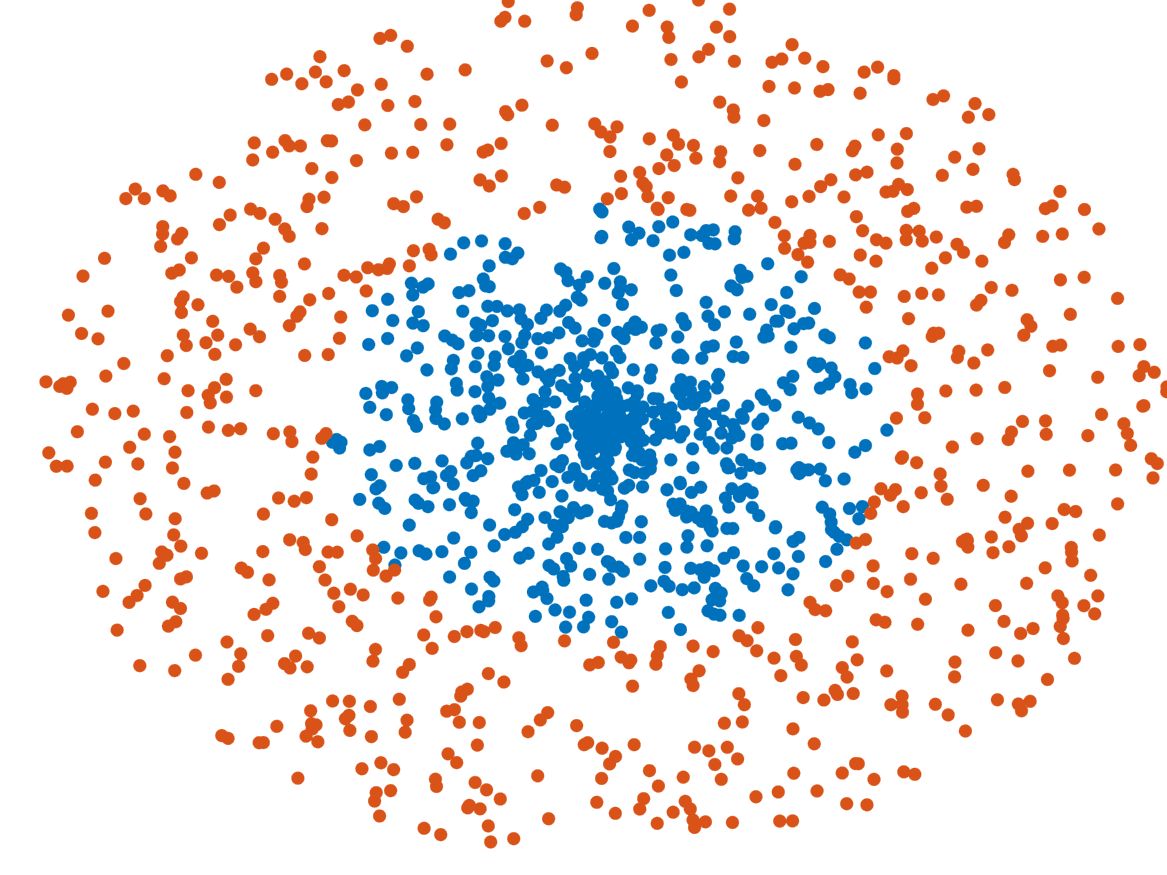
\includegraphics[width=45mm]{Circle-train} & 
		\invisible<beamer|1>{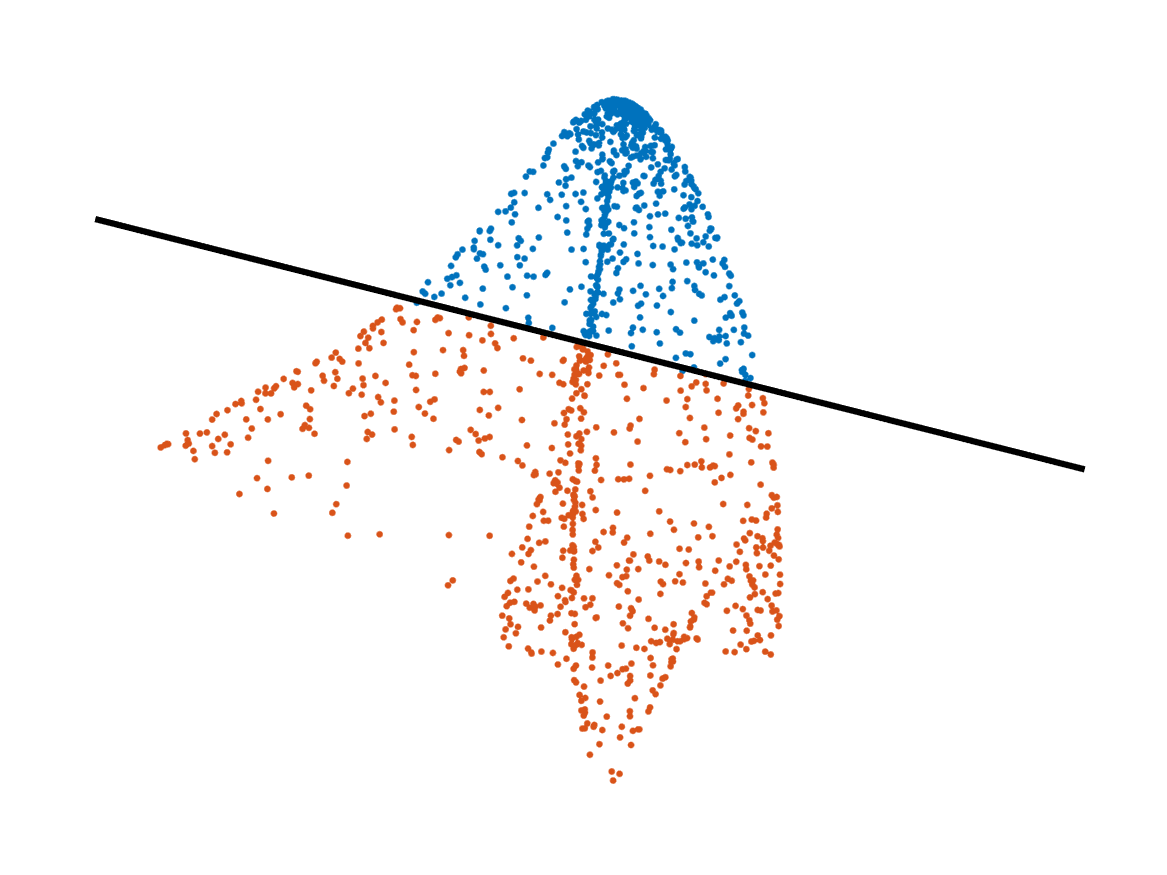
\includegraphics[width=45mm]{Circle-proptrain} }\\
		input features, $\bfY(0)$ & \invisible<beamer|1>{transformed features $\bfY(T)$}
	\end{tabular}
\end{center}
\only<beamer|2>{}
\end{frame}

\begin{frame}[fragile]\frametitle{Residual Network - Forward Propagation}

Idea: Obtain forward propagation by discretizing the ODE

$$ \partial_t{\bfY} = \sigma( \bfK\bfY + b) \quad \bfY(0) = \bfY_0 $$

\bigskip
\pause

Example: Use forward Euler method
\begin{eqnarray*}
\bfY_{j+1} = \bfY_j + h \sigma( \bfK_j\bfY_j + b_j)
\end{eqnarray*}
Here: $\bfY_j$ is called the \emph{state}, $\bfK_j, b_j$ are \emph{controls}, and $h>0$ is time step size.

\bigskip
\pause

More general forward propagation
\begin{eqnarray*}
\bfY_{j+1} =  \bfP_j \bfY_j + h \sigma(\bfK_j\bfY_j  + b_j), \qquad \bfP_j \text{ fixed.}
\end{eqnarray*}
Allows for changing resolution and width (and classical neural networks).


\end{frame}
% section optimization_problem (end)

\section{Computing Derivatives} % (fold)
\begin{frame}[fragile]\frametitle{Residual Network - Classification Problem}


Classification with final state by solving
$$ \min_{\bfW, \bfK_{0,\ldots,N-1},b_{0,\ldots,N-1}}E\left(
\bfW \bfY_N(\bfK_{0,\ldots,N-1},b_{0,\ldots,N-1}),\bfC^{\rm obs}\right) $$

\bigskip
\pause

Need to differentiate
\begin{itemize}
\item $E$ w.r.t $\bfW$ (linear classifier $\leadsto$ Lecture 3)

\item ${\cal S}$ w.r.t $\bfY_N$ (single layer $\leadsto$ Lecture 8)

\item $\bfY_N$ w.r.t control variables ($\bfK_{0,\ldots,N-1},b_{0,\ldots,N-1}$)
\end{itemize}

\bigskip
\pause

Having these, apply chain rule to get, e.g.,
$$
\grad_{\bfK_j} E =  \left(\bfJ_{\bfK_j} {\bfY_N}\right)^{\top} \grad_{\bfY_N} E
$$

How? Adjoint method~\cite{bliss1919,BorzSchulz2012} (more general than back propagation~\cite{Rumelhart1986})
\end{frame}


\begin{frame}[fragile]\frametitle{Computing Derivatives - Sensitivity Equation}
Idea: Differentiate the forward propagation (forward Euler) with respect to $\bfK_i$ for fixed  $0\leq i \leq N$. Note that
$$
	\bfJ_{\bfK_i} \bfY_j = 0, \quad \text{ for } \quad j\leq i. 
$$

\smallskip
\pause

Next, note that 
$$
\bfJ_{\bfK_j} \bfY_{i+1} = h {\rm diag}(\sigma'( \bfK_i \bfY_i + b_i))
(  \bfY_i^\top \otimes \bfI)
$$

\smallskip
\pause

Continuing like this, gives for the final state:
\begin{eqnarray*}
\bfJ_{\bfK_i}\bfY_{N} & =& \bfP_{N-1}  \bfJ_{\bfK_i}\bfY_{N-1}  \\
	&  +& h {\rm diag}(\sigma'( \cdots)) \left( ( \bfI \otimes \bfK_{N-1}) \bfJ_{\bfK_i}\bfY_{N-1}\right) 
\end{eqnarray*}
\smallskip
\pause
Next: Write this as a block triangular {\bf linear} system.
\end{frame}


\begin{frame}[fragile]\frametitle{Computing Derivatives - Sensitivity Equations}

Block triangular {\bf linear} system for the gradients
{\small
\begin{eqnarray*}
\begin{pmatrix}
\bfI              &                &                &          &       \\
-\bfT_{i+1}    &   \bfI       &                &          &       \\
                    & \ddots    &  \ddots    &          &      \\
                    &     &      &          &      \\
                    &     &        &   -\bfT_{N-1}       & \bfI
                    \end{pmatrix}
                    \begin{pmatrix}
                    \bfJ_{\bfK_i}\bfY_{i+1} \\    \\   \\ \\   \bfJ_{\bfK_i}\bfY_{N}
                    \end{pmatrix} =
                    \begin{pmatrix}
                    \bfR_i \\  0\\  \vdots \\ \\   0
                    \end{pmatrix}
\end{eqnarray*}}


$$\bfT_j = \bfP_j + h {\rm diag}(\sigma'( \bfK_j \bfY_j+ b_j))
(\bfI \otimes \bfK_j) $$

and 

$$ \bfR_i = h {\rm diag}(\sigma'(\bfK_i \bfY_i  + b_i)) ( \bfY_i^\top \otimes \bfI). $$


\end{frame}



\begin{frame}[fragile]\frametitle{Computing Derivatives - Sensitivity Equation}

Block triangular {\bf linear} system for the gradients
{\small
\begin{eqnarray*}
	\underbrace{
\begin{pmatrix}
\bfI              &                &                &          &       \\
-\bfT_{i+1}    &   \bfI       &                &          &       \\
                    & \ddots    &  \ddots    &          &      \\
                    &     &      &          &      \\
                    &     &        &   -\bfT_{N-1}       & \bfI
                    \end{pmatrix}}_{=\bfT}
					\underbrace{
                    \begin{pmatrix}
                    \bfJ_{\bfK_i}\bfY_{i+1} \\    \\   \\ \\   \bfJ_{\bfK_i}\bfY_{N}
                    \end{pmatrix}}_{= {\bfJ_{\bfK_i} \bfY}} =
					\underbrace{
                    \begin{pmatrix}
                    \bfR_i \\  0\\  \vdots \\ \\    0
                    \end{pmatrix}}_{=\bfR}
\end{eqnarray*}}

To compute matrix-vector product $(\bfJ_{\bfK_i}\bfY_{N})\, \bfv$
\begin{itemize}
\item Multiply $\bfR\, \bfv$
\item Solve (forward propagate) $\bfT\, \bfJ_{\bfK_i}\bfY = \bfR\, \bfv$
\item Extract the last time step
\end{itemize}

\end{frame}

\begin{frame}[fragile]\frametitle{The Sensitivity Equation}


Symbolically

$$ \bfJ_{\bfK_i}\bfY_{N}  = \bfQ \bfT^{-1}  \bfR  $$
where
$$\bfQ = [0,\ldots,\bfI]. $$


\bigskip

The transpose

$$ \left(\bfJ_{\bfK_i}\bfY_{N}\right)^{\top} =  \bfR^{\top} \bfT^{-T} \bfQ^{\top} $$


\end{frame}

\begin{frame}[fragile]\frametitle{The Sensitivity Equation}

$$ \left(\grad_{\bfK_i}\bfY_{N}\right)^{\top} =  \bfR^{\top} \bfT^{-T} \bfQ^{\top} $$


{\small
\begin{eqnarray*}
\begin{pmatrix} \bfR_i^{\top}  &   0   &  \hdots     &   & 0 \end{pmatrix}
\begin{pmatrix}
\bfI              &  -\bfT_{i+1}^{\top}  &                &          &       \\
                    &   \bfI       &     -\bfT_{i+2}^{\top}           &          &       \\
                    &     &  \ddots    &    \ddots      &      \\
                    &     &      &    \bfI      &  -\bfT_{N}    \\
                    &     &        &          & \bfI
                    \end{pmatrix}^{-1}
  \begin{pmatrix} 0 \\    \\   \vdots  \\    \\  \bfI \end{pmatrix}
\end{eqnarray*}
}



To multiply by the transpose
\begin{itemize}
\item Initialize with last step
\item {\bf solve backward} in time
\item Extract the first step and multiply by $\bfR_i^{\top} $
\end{itemize}

\end{frame}

\begin{frame}[fragile]\frametitle{More about the sensitivity equation}

To compute $({\bfJ_{\bfK_i}}\bfY_N)^{\top} $ for all $i$'s note that the same quantities
are recomputed. Can be evaluated in ${\cal O}(N)$ steps

\bigskip

For gradient based method the transpose is sufficient

\bigskip

Newton based methods require both forward sensitivities and adjoint.


\end{frame}

\begin{frame}[fragile]\frametitle{Testing Derivatives}

{\bf Task 1: Programming the derivative test}

as usual


{\bf Task 2: Programming the adjoint - the adjoint test}

Code a - Computes $(\bfJ_{\bfK_i}\bfY_N)\bfv$

Code b - Computes $(\bfJ_{\bfK_i}\bfY_N)^{\top}\bfu$

\bigskip

Testing - for random $\bfu,\bfv$
$$ \bfu^{\top} \left((\bfJ_{\bfK_i}\bfY_N)\bfv \right) = \bfv^{\top} \left((\bfJ_{\bfK_i}\bfY_N)^{\top}\bfu \right)
$$

\end{frame}
% section computing_derivatives (end)

\begin{frame}[allowframebreaks]
	\frametitle{References}
\bibliographystyle{abbrv}
\bibliography{NumDNN}

\end{frame}
\end{document}
















